\scanpage{135}
\uline{Groupes de Galois motiviques commutatifs.}
\margin{D R}

$k$ corps

$M$ catégorie des (iso)-motifs ($\frac12$ simples) sur $k$

$G$ lien de $M$, \deleted{\unsure{supposé commutatif}}

$\mathscr G$ gerbe des \deleted{\unsure{les}} foncteurs fibres de $M$

$\deleted{\unsure{\mathscr G}}$
\margin{D R}
$\deleted{\unsure{\mathscr G\to}}\quad\uline{M_0\subset M}$, catégorie \deleted{\unsure{des objets}} \inserted{engendrée} par $Q(1)$ de Tate

$\mathscr G_0$, $G_0=G_m$ gerbe et lien correspondants

\diagram{\begin{tikzcd}
\mathscr G \arrow[r] & \mathscr G_0 \\
G \arrow[r,"\varepsilon","\uline{\text{épimorphisme}}"'] & G_m
\end{tikzcd}}
$\mathscr G_0$ est trivialisée i.e. on se donne une section, correspondant à un foncteur-fibre $\varphi$ \deleted{$Q(1)\longrightarrow Q$} choisi sur $M_0$

[\uline{NB} Comme $H^1(Q,G_m)=0$, deux foncteurs fibres sur $M_0$ sont \inserted{\deleted{\unsure{can.}}} isomorphes]
\margin{D R}

Une trivialisation de $\mathscr G_0$ permet de \uline{\unsure{rétrécir|restreindre}} le lien de $\mathscr G$ de $G$ à $\operatorname{Ker}\varepsilon=\unsure{U}$: on prend les foncteurs fibres \uline{munis} d'un isom. de leur restriction à $M_0$ avec le foncteur fibre fixé sur $M_0$. On trouve une nouvelle gerbe $\mathscr G_\varphi$ de lien $U$.
\margin{\uline{\unsure{cf|voir} Giraud?}}
\margin{D R}

Soit $M'$ la ss-catégorie de $M$ formée des objets $M$ tels que les $\otimes^{\unsure{n|\bullet}}(M+\check M)$ soient combinaisons d'un nb fini d'objets simples; \inserted{$\mathscr G'$ la gerbe associée, $G'$ le lien.} On en déduit
\margin{D R}
\diagram{\begin{tikzcd}
& & \mathscr G \arrow[r] & \mathscr G' \arrow[r,dash] & 1 \\
1 \arrow[r,dash] & G^{\unsure{\circ|0}} \arrow[r,dash] & G \arrow[r,"\text{épim}"'] & G' \arrow[r,dash] & 1
\end{tikzcd}}
\margin{D R}
\margin{\figure{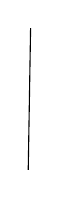
\begin{tikzpicture}\draw (0,0)--(0.03,1.8);\end{tikzpicture}}}
le noyau de $G\to G'$ est la ``composante neutre'' $G^{\unsure{\circ|0}}$.
\margin{D R}

D'autre part, l'on sait que $M'$ est équivalente à une ss-catégorie \inserted{pleinement fidèle} des $Q$-\unsure{vectoriels} étales sur $k$. La donnée d'une clôture algébrique $\overline k$ de $k$ fournit un
\margin{D R}
\mspage{134}
